\section{Success probabilities and an exact constrained dual}
\label{sec:ext-probability}

An optimum conditional CHSH value does not determine a unique success
probability, because a Kraus operator may be scaled down arbitrarily.
Throughout this section, $p_{\max}$ denotes the largest probability
compatible with $F^\dagger F\le I$ for the specified conditional filter.

\begin{proposition}[Exact maximal success probability]
\label{prop:ext-success}
For a canonical effect $I+u\cdot\sigma$,
\begin{equation}
 p_{\max}(0,u)=\frac1{1+\norm u}.
 \label{eq:ext-canonical-success}
\end{equation}
For the original mixed Alice marginal with Bloch vector $a$, the
whitening-and-filtering branch
$F=\sqrt{I+u\cdot\sigma}\,(I+a\cdot\sigma)^{-1/2}$
has
\begin{equation}
 \boxed{
 p_{\max}(a,u)=
 \frac{1-\norm a^2}
 {1-a\cdot u+
 \sqrt{(1-a\cdot u)^2-(1-\norm a^2)(1-\norm u^2)}}.
 }
 \label{eq:ext-original-success}
\end{equation}
\end{proposition}

\begin{proof}
The unscaled branch has success normalization one. If $E=F^\dagger F$,
its largest allowed scalar rescaling has squared size
$1/\lambda_{\max}(E)$, and hence this is its maximum probability.
For a canonical input the effect eigenvalues are $1\pm\norm u$.
For the original state,
\[
 \tr E=\frac{2(1-a\cdot u)}{1-\norm a^2},
 \qquad
 \det E=\frac{1-\norm u^2}{1-\norm a^2}.
\]
The quadratic formula for the larger eigenvalue gives
\eqref{eq:ext-original-success}.
\end{proof}

The next theorem concerns the probability constraint on the
\emph{canonical input}. This restriction is substantive: whitening a
general input changes success probabilities, and
\eqref{eq:ext-original-success}, not~\eqref{eq:ext-canonical-success},
must be used when imposing a probability constraint on the original
state.

\begin{theorem}[One-dimensional convex dual for a success constraint]
\label{thm:ext-success-dual}
Suppose $H_0=K+iC\succ0$, which holds in particular when $\alpha>1$.
Require a canonical filter to have maximum success probability at least
$p_0\in[1/2,1]$, and put
$R=p_0^{-1}-1\in[0,1]$.
Let $S_R$ be the largest squared CHSH value under that constraint.
Then
\begin{equation}
 \boxed{
 S_R=\inf_{\tau\ge0}
 \left[
 \tr A+\tau R^2
 -\lambda_{\min}\!\left(A+C(K+\tau I)^{-1}C\right)
 \right].
 }
 \label{eq:ext-success-dual}
\end{equation}
The function minimized is convex in $\tau$.
For $R>0$ it has a finite minimizer, and a corresponding optimal
filter can be reconstructed from its minimum eigenspace.
The value is nondecreasing and concave as a function of $R^2$.
It reaches the unconstrained plateau at
\begin{equation}
 R_*^2=
 \min_{\substack{\norm n=1\\Mn=\lambda_{\min}(M)n}}
       \norm{K^{-1}Cn}^2.
 \label{eq:ext-plateau-radius}
\end{equation}
At $R=0$, $S_0=\tr A-\lambda_{\min}(A)$ is the original canonical
CHSH value.
\end{theorem}

\begin{proof}
The probability constraint is exactly $\norm u\le R$.
The Lorentz reduction in the proof of the main theorem respects it.
Indeed its replacement filter has squared effect norm
$1-1/\Delta$, whereas the original filter has squared effect norm
$1-1/w_0^2$, and $\Delta\le w_0^2$.
Thus replacement decreases the norm and cannot lower the chosen
correlation-plane value. Conversely each reduced feasible pair gives
$u=-n\times v$ with $\norm u=\norm v$.
It follows that $S_R$ is exactly the maximum of $f(n,v)$ subject to
$\norm n=1$, $n\cdot v=0$, and $\norm v\le R$.

For $\tau\ge0$, write
$P_\tau=K+\tau I$ and $M_\tau=A+CP_\tau^{-1}C$.
Completing the square gives, for every feasible pair,
\begin{align}
 f(n,v)
 ={}&\tr A-n^TM_\tau n+\tau\norm v^2 \notag\\
    &-(v+P_\tau^{-1}Cn)^TP_\tau
                  (v+P_\tau^{-1}Cn)
 \le\tr A+\tau R^2-\lambda_{\min}(M_\tau).
 \label{eq:ext-dual-square}
\end{align}
This proves weak duality. The expression on the right is also the
maximum, over $\norm n=1$ and arbitrary real $v$, of
$f(n,v)+\tau(R^2-\norm v^2)$, with the orthogonality constraint
temporarily omitted. It is therefore a supremum of affine functions
of $\tau$, and is convex. For $R>0$ it tends to infinity as
$\tau\to\infty$, so it has a minimizer.

Let $N_\tau$ have orthonormal columns spanning the minimum eigenspace
of $M_\tau$.
The possible squared norms of
$v=-P_\tau^{-1}Cn$, for unit $n$ in that eigenspace, form the whole
Rayleigh interval
\begin{equation}
 [r_-^2(\tau),r_+^2(\tau)]
 =\left[
 \lambda_{\min}(N_\tau^TC^TP_\tau^{-2}CN_\tau),
 \lambda_{\max}(N_\tau^TC^TP_\tau^{-2}CN_\tau)
 \right].
 \label{eq:ext-radius-interval}
\end{equation}
Here $M_\tau'=-CP_\tau^{-2}C=C^TP_\tau^{-2}C$.
The left and right derivatives of the convex dual function are
$R^2-r_+^2(\tau)$ and $R^2-r_-^2(\tau)$, respectively.
At a positive minimizing $\tau$, they bracket zero, so choose a unit
minimum eigenvector whose associated $v$ has norm exactly $R$.
At a minimizer $\tau=0$, the right derivative is nonnegative,
so choose one with $\norm v\le R$.

It remains to check the omitted orthogonality condition.
The positive matrix $H_0+\tau I=P_\tau+iC$ has Schur complement
\[
 P_\tau+CP_\tau^{-1}C
 =M_\tau+(\tau-s)I\succ0.
\]
The paired eigenvector equations therefore force
$(\lambda_{\min}(M_\tau)+\tau-s)n\cdot v=0$ with a strictly
positive coefficient, so $n\cdot v=0$.
The selected pair is feasible and gives equality in
\eqref{eq:ext-dual-square}, proving strong duality.
This argument uses the entire eigenspace and therefore includes
eigenvalue crossings.

The infimum of affine functions of $R^2$ is concave; monotonicity
also follows directly from nesting of the feasible balls.
At $\tau=0$, the same one-sided derivative test is precisely
$R^2\ge R_*^2$, proving the plateau assertion.
For $R=0$, the primal domain forces $v=0$, and the dual tends to
the same value as $\tau\to\infty$.
\end{proof}

Equation~\eqref{eq:ext-success-dual} is an exact convex scalar
representation. In general it is not asserted to be a formula in
radicals. The axial family does permit a complete piecewise expression,
including an interval where the best filter breaks the apparent axial
symmetry.

\begin{theorem}[Closed axial frontier and tilted optimal filters]
\label{thm:ext-axial-frontier}
For~\eqref{eq:ext-axial-family}, suppose $H_0\succ0$, and put
\[
 k=x-c_0^2,\qquad g=rc_0>0,\qquad R_*=\frac gk<1.
\]
If $x\le r^2$, then
\begin{equation}
 S_R=
 \begin{cases}
  x+r^2+2gR-kR^2,&0\le R\le R_*,\\
  x+r^2+g^2/k,&R\ge R_*.
 \end{cases}
 \label{eq:ext-axial-frontier-first}
\end{equation}
If $x>r^2$ and $g^2\le k(x-r^2)$, then $S_R=2x$ for every $R$.
In the remaining case, define
\[
 \tau_c=\frac{g^2}{x-r^2}-k>0,\qquad
 R_c=\frac{x-r^2}{g},\qquad 0<R_c<R_*.
\]
Then
\begin{equation}
 \boxed{
 S_R=
 \begin{cases}
 2x+\tau_cR^2,&0\le R\le R_c,\\
 x+r^2+2gR-kR^2,&R_c\le R\le R_*,\\
 x+r^2+g^2/k,&R\ge R_*.
 \end{cases}}
 \label{eq:ext-axial-frontier}
\end{equation}
For $0<R<R_c$, one optimal effect is
\begin{equation}
 u=\left(-R\sqrt{1-(R/R_c)^2},\,0,\,R^2/R_c\right),
 \label{eq:ext-tilted-effect}
\end{equation}
up to rotations about the symmetry axis. Every optimal effect in this
open interval has a nonzero component perpendicular to that axis.
For $R_c\le R\le R_*$, an optimal effect is $u=(0,0,R)$; above
the plateau, replace $R$ by $R_*$.
\end{theorem}

\begin{proof}
Positivity of $H_0$ is equivalent here to $k>g$ and $r^2>c_0^2$.
The eigenvalues of $M_\tau$ are
$x-g^2/(k+\tau)$, twice, and $r^2$.
Consequently the dual objective is the \emph{upper} envelope
\begin{equation}
 \max\left\{
 x+r^2+\tau R^2+\frac{g^2}{k+\tau},\
 2x+\tau R^2
 \right\}.
 \label{eq:ext-axial-dual-envelope}
\end{equation}
If $x\le r^2$, the first branch is always active. Its minimizing
parameter for $R>0$ is $\tau=\max(g/R-k,0)$, yielding
\eqref{eq:ext-axial-frontier-first}; at $R=0$ the infimum is
obtained as $\tau\to\infty$.
If $x>r^2$ but $\tau_c\le0$, the second branch is always active,
and $\tau=0$ gives the constant value $2x$.

In the remaining case the first branch applies for
$0\le\tau\le\tau_c$, and the second for $\tau\ge\tau_c$.
For $0<R<R_c$ their left and right slopes at the crossing have
opposite signs, so the minimum is at $\tau_c$.
At $R=0$, every $\tau\ge\tau_c$ has the minimum value $2x$.
For $R_c\le R\le R_*$ it is at $\tau=g/R-k$;
for $R\ge R_*$ it is at zero. Substitution proves all three pieces.

At $\tau_c$, the minimum eigenspace is all of $\R^3$.
Set $\theta=(R/R_c)^2$ and choose
\[
 n=(\sqrt\theta,0,\sqrt{1-\theta}),\qquad
 v=(0,-R_c\sqrt\theta,0).
\]
These vectors satisfy $\norm n=1$, $n\cdot v=0$, and $\norm v=R$,
and give~\eqref{eq:ext-tilted-effect}.
Moreover every equality pair must have
$v=-(K+\tau_cI)^{-1}Cn$ and $\norm v=R$.
It follows that the transverse squared norm of $n$ is $\theta$,
so $\norm{u_\perp}=R\sqrt{1-\theta}>0$.
Thus a restriction to axial effects loses the true optimum throughout
this interval.
\end{proof}

\subsection{An exact probability threshold inside the tilted regime}

Return to the canonical activation example
$\rho_1=\tfrac1{40}\left(\begin{smallmatrix}
20&0&0&14\\0&0&0&0\\0&0&7&0\\14&0&0&13
\end{smallmatrix}\right)$ from the earlier examples.
Here
\[
 x=\frac{49}{100},\quad r=\frac{13}{20},\quad c_0=\frac7{20},
 \quad k=\frac{147}{400},\quad g=\frac{91}{400}.
\]
The exact breakpoints and scalar dual parameter are
\[
 R_c=\frac{27}{91},\qquad
 R_*=\frac{13}{21},\qquad
 \tau_c=\frac{539}{1350}.
\]
Thus
\begin{equation}
 S_R=
 \begin{cases}
 \displaystyle\frac{49}{50}+\frac{539}{1350}R^2,
       &0\le R\le27/91,\\[3pt]
 \displaystyle\frac{73}{80}+\frac{91}{200}R-\frac{147}{400}R^2,
       &27/91\le R\le13/21,\\[3pt]
 \displaystyle\frac{79}{75},&R\ge13/21.
 \end{cases}
 \label{eq:ext-exact-frontier}
\end{equation}
The constrained state violates CHSH exactly when
\begin{equation}
 R>\sqrt{\frac{27}{539}}
 \quad\Longleftrightarrow\quad
 p_0<\frac1{1+\sqrt{27/539}}.
 \label{eq:ext-success-threshold}
\end{equation}
Since $\sqrt{27/539}<27/91$, the first onset of violation occurs
strictly inside the tilted-filter regime. This is a concrete obstruction
to optimizing the success tradeoff by assuming that an axially symmetric
input has an axial optimal filter.

\begin{figure}[tbp]
 \centering
 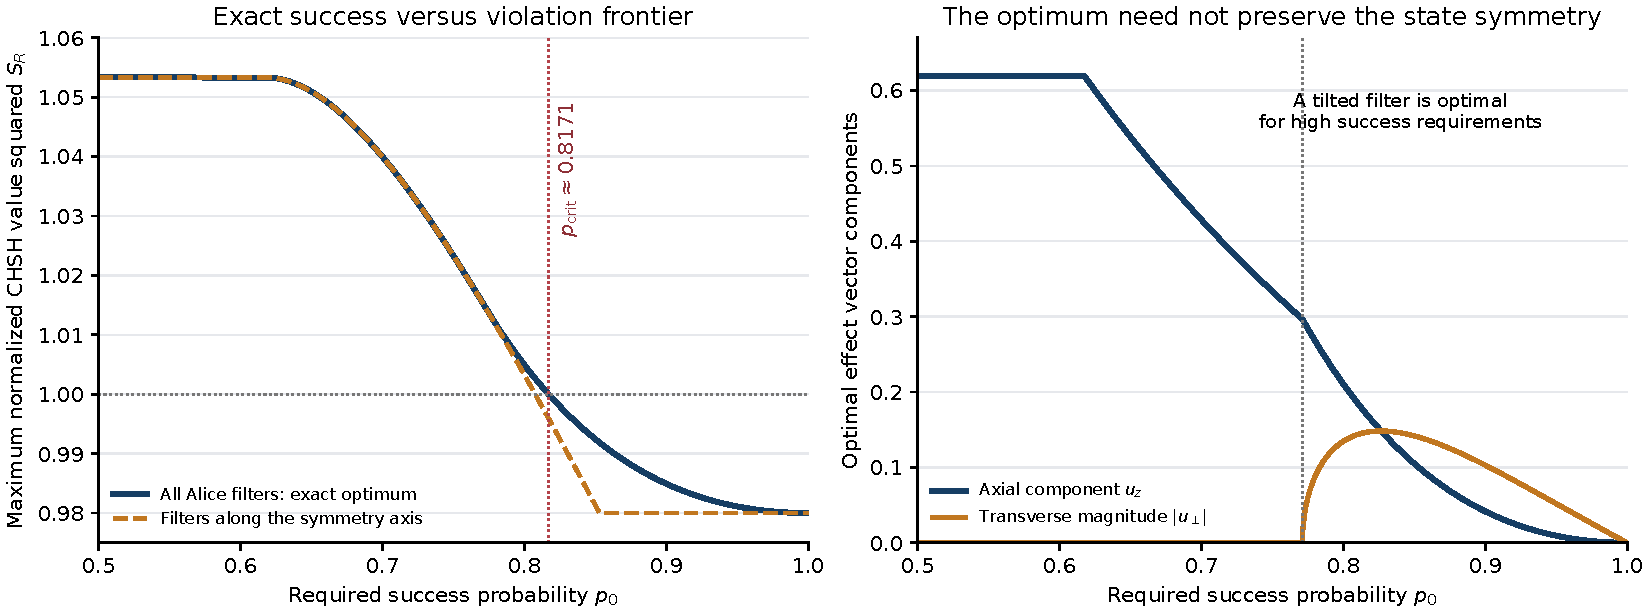
\includegraphics[width=\linewidth]{figures/exact_success_frontier.pdf}
 \caption{The exact success frontier for $\rho_1$.
 Left: the unrestricted optimum~\eqref{eq:ext-exact-frontier}
 compared with filters constrained to the symmetry axis.
 Right: the axial and transverse components of an optimal effect.
 A nonzero transverse component is necessary throughout the high-success
 interval corresponding to $0<R<R_c$.}
 \label{fig:ext-success-frontier}
\end{figure}


\section{Success constraints on the original input state}
\label{sec:r3-success}

The earlier scalar dual constrains the success probability on a canonical
input. Whitening is itself probabilistic, so that dual does not directly
solve the tradeoff on the original state. This section gives the correct
feasible geometry, an exact algebraic optimization for every input, and
closed frontiers for several noncanonical families.

Let the original Alice marginal have Bloch vector $a$, with
$r=\norm a<1$, and put $W=(I+a\cdot\sigma)^{-1/2}$.
Write the canonical data as $(c,D)$ and set $Q=D^TD$.
For $0\le p\le1$, define
\[
 S_\rho(p)=
 \sup_{\substack{F\text{ invertible},\ F^\dagger F\preceq I\\
                  \tr[(F^\dagger F\otimes I)\rho]\ge p}}
 B(\rho_F)^2.
\]
Thus $p$ is a required success probability, rather than the probability
of a particular arbitrarily rescaled Kraus operator.

\subsection{Two balls, rather than a centered-radius constraint}

\begin{theorem}[Exact original-input success lens]
\label{thm:r3-lens}
A canonical effect vector $u$, $\norm u\le1$, can be implemented on the
original state with success probability at least $p$ if and only if
\begin{equation}
 \boxed{\qquad \norm{a-pu}\le1-p.\qquad}
 \label{eq:r3-lens}
\end{equation}
Consequently its feasible set is
\begin{equation}
 \mathcal L_p(a)=
 \{u:\norm u\le1,\ \norm{a-pu}\le1-p\}.
 \label{eq:r3-lens-set}
\end{equation}
For $p>0$, the second condition is the ball centered at $a/p$ of
radius $(1-p)/p$. The constraint is inactive when
$p\le(1-r)/2$. That second ball lies inside the unit ball when
$p\ge(1+r)/2$. At $p=1$ the lens is the singleton $\{a\}$.

The smallest and largest feasible norms are
\begin{equation}
 r_-(p)=\max\left\{0,1-\frac{1-r}{p}\right\},\qquad
 r_+(p)=\min\left\{1,\frac{1+r}{p}-1\right\},
 \label{eq:r3-radius-range}
\end{equation}
with $r_-(0)=0$ and $r_+(0)=1$.
\end{theorem}

\begin{proof}
The unscaled combined filter is
$F_u=\sqrt{I+u\cdot\sigma}\,W$, and its success normalization on
$\rho$ is one. Its largest physical success probability is
$1/\lambda_{\max}(E_u)$, where
$E_u=W(I+u\cdot\sigma)W$. Hence success at least $p$ is equivalent to
$pE_u\preceq I$. Congruence by $W^{-1}$ turns this into
\[
 p(I+u\cdot\sigma)\preceq I+a\cdot\sigma.
\]
The difference has eigenvalues $1-p\pm\norm{a-pu}$, proving
\eqref{eq:r3-lens}.
The two ball-containment conditions follow by comparing their center
distance $r/p$ and radii $1,(1-p)/p$.

The nearest point of the second ball to the origin has distance
$\max(0,[r-(1-p)]/p)=r_-(p)$, and it lies in the unit ball since
$r_-(p)\le r<1$.
The farthest feasible distance is the smaller of one and the second
ball's farthest distance $(r+1-p)/p$.
Both extrema are obtained on the line through $a$; if $a=0$, any
radial direction may be used for the maximum.
\end{proof}

In particular, whitening $u=0$ is allowed exactly when $p\le1-r$,
which is a different threshold from the condition that \emph{every}
canonical filter is allowed.

\begin{figure}[htbp]
\centering
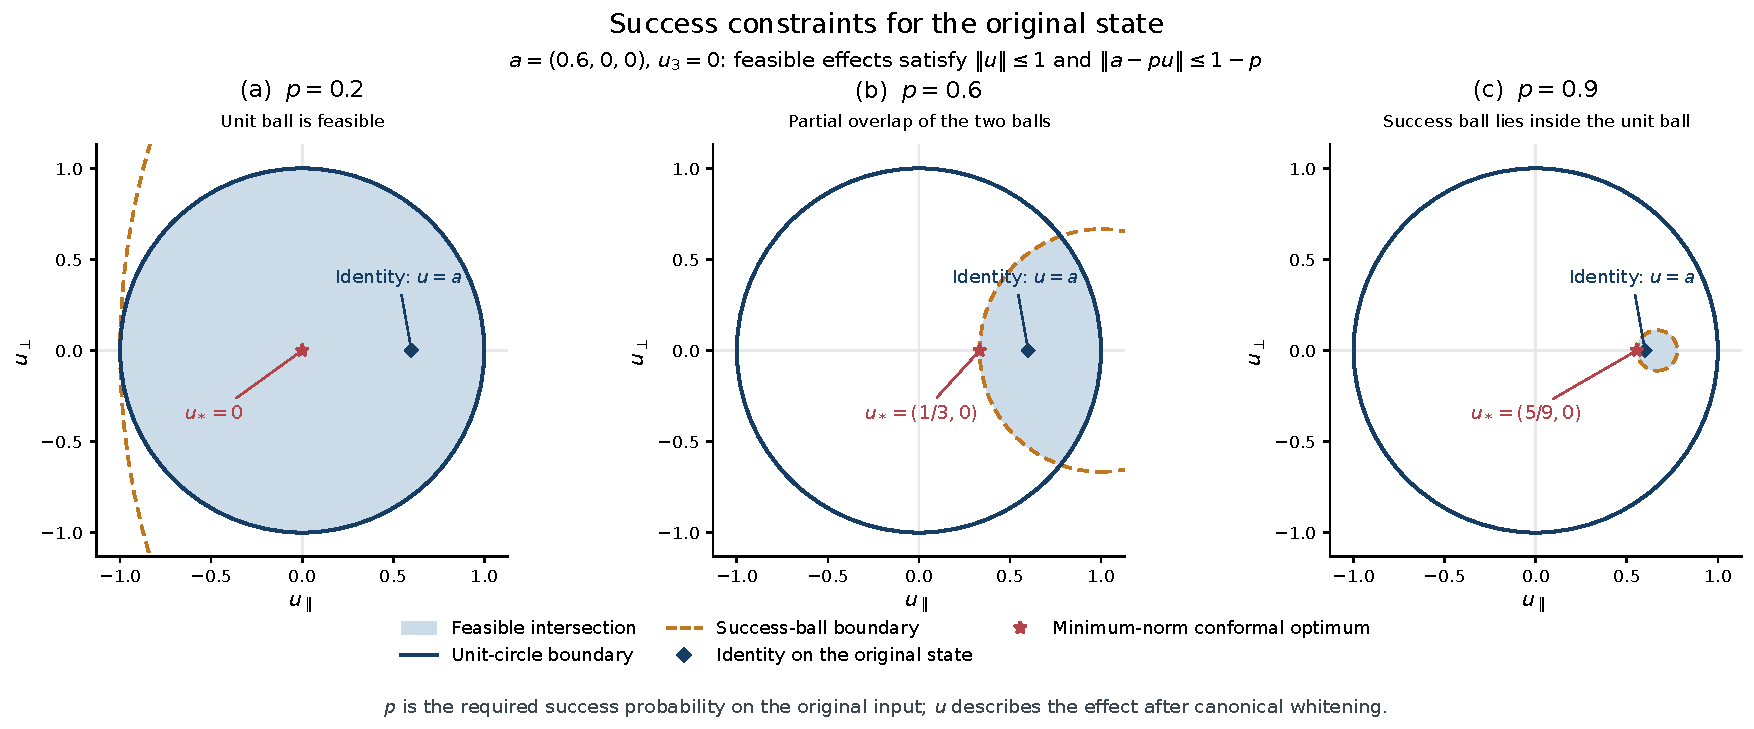
\includegraphics[width=\textwidth]{figures/original_success_lens.pdf}
\caption{Planar sections of the exact original-input success lens at
$\norm a=0.6$. As the required probability increases, the feasible region
changes from the entire effect ball to a lens and then to a smaller ball.
The identity filter on the original state corresponds to $u=a$ and remains
feasible. The closest point to the origin
is the exact optimum for the conformal family of Theorem~\ref{thm:r3-conformal}.}
\label{fig:r3-lens}
\end{figure}

\begin{lemma}[Density of invertible filters and attainment above one]
\label{lem:r3-density}
Maximizing a continuous filtered score over the closed lens gives the
same value as the invertible-filter supremum.
Every constrained optimum with $S_\rho(p)>1$ is attained by an
invertible filter.
\end{lemma}

\begin{proof}
For $p<1$, the point $u=a$ is strictly inside both defining balls:
$\norm a<1$ and $\norm{a-pa}=(1-p)r<1-p$.
For any feasible $u$, the points $u_t=(1-t)u+ta$, $0<t\le1$,
remain feasible by convexity and satisfy $\norm{u_t}<1$.
They converge to $u$, so invertible effects are dense.
At $p=1$, the only feasible point is already the interior point $a$.
Finally, $\norm u=1$ gives a rank-one Alice filter and therefore a
product output, whose normalized CHSH value is at most one.
A compact maximizer with value greater than one must consequently
have $\norm u<1$.
\end{proof}

\subsection{The correct quadratic Gram matrix}

\begin{theorem}[An exact three-variable constrained optimization]
\label{thm:r3-gram}
Define the polynomial symmetric matrix
\begin{equation}
 \boxed{
 G(u)=(1-\norm u^2)(Q-cc^T)
             +(c+D^Tu)(c+D^Tu)^T.
 }
 \label{eq:r3-bob-gram}
\end{equation}
Then, for every canonical effect including $\norm u=1$,
$G(u)=T_u^TT_u$. In particular
\begin{equation}
 \boxed{
 S_\rho(p)=\max_{u\in\mathcal L_p(a)}
       [\,\tr G(u)-\lambda_{\min}(G(u))\,].
 }
 \label{eq:r3-primal}
\end{equation}
Equivalently, for each unit Bob-side normal $n$, put $P_n=I-nn^T$,
\[
 k_n=\tr[P_n(Q-cc^T)],\qquad
 h_n=DP_nc,\qquad J_n=k_nI-DP_nD^T.
\]
The objective associated with that measurement plane is the quadratic
\begin{equation}
 f_n(u)=\tr(P_nQ)+2h_n^Tu-u^TJ_nu,
 \qquad
 S_\rho(p)=\max_{\norm n=1}\max_{u\in\mathcal L_p(a)}f_n(u).
 \label{eq:r3-plane-quadratic}
\end{equation}
\end{theorem}

\begin{proof}
Set $q=\sqrt{1-\norm u^2}$ and
$S_u=qI+uu^T/(1+q)$.
The filtered correlation matrix is $T_u=S_uD+uc^T$.
The identities $S_uu=u$ and $S_u^2=(1-\norm u^2)I+uu^T$
give
\[
 T_u^TT_u=(1-\norm u^2)Q
  +(D^Tu)(D^Tu)^T+(D^Tu)c^T+c(D^Tu)^T+\norm u^2cc^T,
\]
which is~\eqref{eq:r3-bob-gram}. This calculation remains valid at
the rank-one boundary. The Horodecki formula gives
\eqref{eq:r3-primal}; compactness and
Lemma~\ref{lem:r3-density} justify the maximum.
Taking $\tr(P_nG(u))$ and expanding proves
\eqref{eq:r3-plane-quadratic}.
\end{proof}

The Bob-side normal in~\eqref{eq:r3-plane-quadratic} is unrestricted.
It must not be constrained to be perpendicular to $u$.
The Lorentz replacement in the unconstrained proof can change the
effect vector toward the origin, which need not preserve a ball centered
at $a/p$.

\begin{remark}[An exact counterexample to the naive shifted reduction]
\label{rem:r3-counterexample}
Take the full-rank original state
\begin{equation}
 \rho=\frac1{200}
 \begin{pmatrix}
 116&0&0&56\\0&44&8&0\\0&8&11&0\\56&0&0&29
 \end{pmatrix}.
 \label{eq:r3-counterexample}
\end{equation}
The two block determinants before division by $200^2$ are $228$ and
$420$, so positivity is strict. Here $a=(0,0,3/5)$, and the canonical
data are $c=0$, $D=\diag(4/5,-3/5,9/20)$.
Thus $K=DD^T\succ0$ and $\alpha=481/400>1$.
At $p=1$, only $u=a$ is feasible, and the true score is
$S_\rho(1)=16/25$.
If one instead imposes $u=-n\times v=a$ in the earlier reduced
objective, one forces $n\perp a$ and obtains only
\[
 (16/25)^2+(9/20)^2=\frac{6121}{10000}
 <\frac{16}{25}.
\]
The failure therefore occurs even inside the positive-Gram regime.
\end{remark}

\subsection{A rational description using the ellipsoid and original marginals}

\begin{theorem}[The full frontier needs no canonical orientation]
\label{thm:r3-ellipsoid}
Let $b$ be the original Bob Bloch vector, $g=b-c=D^Ta$, and
$Q=D^TD$. If $Q\succ0$, set $w=D^Tu$. Then the exact frontier is
obtained by maximizing the top-two eigenvalue sum of
\begin{equation}
 \mathcal G(w)=
 (1-w^TQ^{-1}w)(Q-cc^T)+(c+w)(c+w)^T
 \label{eq:r3-ellipsoid-gram}
\end{equation}
under the two ellipsoid constraints
\begin{equation}
 w^TQ^{-1}w\le1,\qquad
 (g-pw)^TQ^{-1}(g-pw)\le(1-p)^2.
 \label{eq:r3-two-ellipsoids}
\end{equation}
All coefficients are rational functions of the original Bloch data.

The same statement extends to singular $Q$ as follows.
Write $Q^\dagger$ for its Moore--Penrose inverse, restrict
$w\in\ran Q$, and put
\[
 \eta=\norm a^2-g^TQ^\dagger g\ge0.
\]
If $\rank Q<3$ and $\eta>0$, introduce $k\ge0$ and set
\begin{align}
 q&=w^TQ^\dagger w+k^2/\eta,\\
 \ell&=(g-pw)^TQ^\dagger(g-pw)
              +\eta-2pk+p^2k^2/\eta.
 \label{eq:r3-singular-positive}
\end{align}
If $\rank Q<3$ and $\eta=0$, introduce $t\ge0$ and instead set
\begin{equation}
 q=w^TQ^\dagger w+t,\qquad
 \ell=(g-pw)^TQ^\dagger(g-pw)+p^2t.
 \label{eq:r3-singular-zero}
\end{equation}
In both cases maximize the top-two eigenvalue sum of
\begin{equation}
 (1-q)(Q-cc^T)+(c+w)(c+w)^T
 \label{eq:r3-singular-gram}
\end{equation}
under $q\le1$ and $\ell\le(1-p)^2$.
This is exact, including all rank-zero, rank-one, and rank-two shapes.
After choosing coordinates in $\ran Q$, it uses at most three real
variables and has rational coefficients on each rank stratum.
\end{theorem}

\begin{proof}
When $D$ is invertible, $u=D^{-T}w$ and $a=D^{-T}g$, proving
\eqref{eq:r3-two-ellipsoids} and~\eqref{eq:r3-ellipsoid-gram}.
The equality $g=b-c$ follows by applying the effect $u=a$, which
undoes whitening and restores the original Bob marginal.
Alternatively it follows directly from
$c=(b-T^Ta)/(1-\norm a^2)$.

For the singular case decompose orthogonally
\[
 u=DQ^\dagger w+u_0,\qquad
 a=DQ^\dagger g+a_0,\qquad
 u_0,a_0\in\ker D^T.
\]
Then $\norm{a_0}^2=\eta$ and
$\norm u^2=w^TQ^\dagger w+\norm{u_0}^2$.
The Gram matrix depends on $u_0$ only through its squared norm.
For a fixed norm, the smallest possible value of
$\norm{a_0-pu_0}^2$ is obtained by aligning $u_0$ with $a_0$.
If $\eta>0$, write $u_0=(k/\eta)a_0$ with $k\ge0$.
Its norm and distance are exactly the extra terms
in~\eqref{eq:r3-singular-positive}.
If $\eta=0$, choose any null-space vector of squared norm $t$,
giving~\eqref{eq:r3-singular-zero}.
This alignment preserves the score and can only improve success
feasibility; every reduced feasible point reconstructs a real filter.

The raw formulas for $c,Q$ are rational, as in
\eqref{eq:ext-raw-ellipsoid}. The pseudoinverse is rational on each
rank stratum. Explicitly, with $e_1=\tr Q$ and
$e_2=((\tr Q)^2-\tr Q^2)/2$,
\[
 Q^\dagger=
 \begin{cases}
 0,&\rank Q=0,\\
 Q/e_1^2,&\rank Q=1,\\
 [(e_1^2-e_2)Q-e_1Q^2]/e_2^2,&\rank Q=2,\\
 \adj(Q)/\det Q,&\rank Q=3.
 \end{cases}
\]
Each formula follows by evaluation on the nonzero eigenvalues.
For rank below three, there are $\rank Q$ range coordinates and one
additional scalar, proving the dimension bound.
\end{proof}

This theorem says precisely which extra data the original-input
tradeoff needs: the steering ellipsoid $(Q,c)$, the original Bob point
$b$, and the length $\norm a$. In the nonsingular case the latter is
already encoded by $g^TQ^{-1}g$.
The conditional Bob Bloch vector is $c+w$; the second ellipsoid
constraint is the condition that the complementary outcome can also
have a conditional Bob vector in the same ellipsoid.

\subsection{Exact algebraic decisions and verifiable upper certificates}

\begin{proposition}[Degree-six decision and a complete certificate hierarchy]
\label{prop:r3-certificates}
For a proposed squared-score threshold $\gamma$, define
\[
 H_\gamma(u)=\gamma I-\tr G(u)I+G(u),\quad
 g_1(u)=1-\norm u^2,\quad
 g_2(u)=(1-p)^2-\norm{a-pu}^2.
\]
Then $S_\rho(p)>\gamma$ exactly when there is a real $u$ with
$g_1,g_2\ge0$ for which at least one of
\begin{equation}
 \tr H_\gamma,\qquad
 \frac{(\tr H_\gamma)^2-\tr(H_\gamma^2)}2,\qquad
 \det H_\gamma
 \label{eq:r3-polynomial-decision}
\end{equation}
is negative. These are polynomials of degree at most $2,4,6$ in
the three coordinates of $u$. Thus real quantifier elimination gives
an exact algebraic decision for algebraic input data.

An exact polynomial identity
\begin{equation}
 H_\gamma=\Sigma_0+g_1\Sigma_1+g_2\Sigma_2,
 \qquad \Sigma_j=\sum_\ell V_{j\ell}^TV_{j\ell},
 \label{eq:r3-sos-certificate}
\end{equation}
is a sufficient upper certificate $S_\rho(p)\le\gamma$.
For every strict upper threshold $\gamma>S_\rho(p)$, such a
matrix sum-of-squares certificate exists at some finite degree.
\end{proposition}

\begin{proof}
The largest eigenvalue of $\tr G\,I-G$ is the sum of the two largest
eigenvalues of $G$. Thus $H_\gamma\succeq0$ is exactly the
pointwise upper-score condition. The three elementary symmetric
coefficient test for a real symmetric $3\times3$ matrix proves
\eqref{eq:r3-polynomial-decision}; the degree bounds follow because
$G$ is quadratic in $u$.

Every right-hand term in~\eqref{eq:r3-sos-certificate} is positive
semidefinite on the lens, proving sufficiency by direct evaluation.
For completeness, if $\gamma>S_\rho(p)$, then $H_\gamma$ is
uniformly positive definite on the compact lens.
The matrix Positivstellensatz of Hol--Scherer~\cite{holscherer2005}
applies: the quadratic module is Archimedean because it already
contains $1-\norm u^2$.
It supplies the displayed representation. No fixed degree is asserted,
and at equality $\gamma=S_\rho(p)$ finite-degree attainment is not
guaranteed.
\end{proof}

Thus one may search for upper certificates by semidefinite programming,
but floating-point feasibility alone is not a certificate: the
polynomial identity and the positive semidefinite Gram matrices must
be checked exactly or with rigorous error bounds. Likewise, the
general-purpose multistart optimizer supplied with this report only
produces numerical candidates. It is not an exact replacement for
quantifier elimination or a verified certificate.

There is additional convex structure for a \emph{fixed} Bob plane.
If $K\succ0$, then $J_n\succ0$ for every $n$: the two nonzero
eigenvalues of $DP_nD^T$ are those of $Q$ restricted to the plane,
so its largest eigenvalue subtracted from $k_n$ leaves at least
$\lambda_{\min}(Q)-\norm c^2>0$.
For $p<1$, strict feasibility at $u=a$ gives the exact inner dual
\begin{align}
 \max_{u\in\mathcal L_p(a)} f_n(u)
 =\min_{\lambda,\mu\ge0}\bigl\{
 &\tr(P_nQ)+\lambda+\mu[(1-p)^2-r^2]\notag\\
 &+(h_n+\mu p a)^T
 [J_n+(\lambda+\mu p^2)I]^{-1}
 (h_n+\mu p a)\bigr\}.
 \label{eq:r3-fixed-plane-dual}
\end{align}
This follows by completing the square and the ordinary strictly
feasible concave quadratic-program duality theorem.
It does not justify interchanging the outer maximum over $n$ with
the dual minimum. No universal scalar dual for the original-state
frontier is claimed here.

\subsection{Universal purity bounds and exact closed families}

Let $\alpha=\tr(DD^T)-\norm c^2$ and $m=(\alpha-1)/2$.
For clarity, the pointwise inequality needed here concerns the
\emph{actual effect} $u$, without any replacement by a reduced
Lorentz pair:
\begin{equation}
 B((\rho_c)_u)^2\le 1+m(1-\norm u^2).
 \label{eq:r3-pointwise-purity}
\end{equation}
One direct proof is as follows. For an arbitrary physical state
$\omega$ with Bloch data $(a',b',T')$, a real unit vector $n$, and
$S_n=(n\cdot\sigma)\otimes I$, Pauli orthogonality gives
\begin{align*}
 4\tr(\omega S_n\widetilde\omega S_n)
 ={}&1+\norm{a'}^2-\norm{b'}^2-\norm{T'}_F^2\\
 &-2(n\cdot a')^2+2n^TT'T'^Tn\ge0.
\end{align*}
The inequality holds because both $\omega$ and
$S_n\widetilde\omega S_n$ are positive semidefinite. Therefore each
Alice measurement-plane score satisfies
\[
 \tr(T'T'^T)-n^TT'T'^Tn
 \le\frac{1+\norm{T'}_F^2+\norm{a'}^2-\norm{b'}^2}{2}
       -(n\cdot a')^2.
\]
For the actual canonical effect, $a'=u$, $b'=c+D^Tu$, and
\eqref{eq:r3-bob-gram} gives
\[
 \norm{T'}_F^2+\norm u^2-\norm{b'}^2
   =\alpha+(1-\alpha)\norm u^2.
\]
Taking the maximum over measurement planes and dropping the
nonnegative square proves~\eqref{eq:r3-pointwise-purity}, including
$\norm u=1$. This is the quantitative purity bound from
Proposition~\ref{prop:ext-purity}, now written entirely in the
coordinates of the constrained problem.

Combining it with the exact norm range of the lens yields
\begin{equation}
 S_\rho(p)\le
 \begin{cases}
 1+m[1-r_-(p)^2],&m\ge0,\\
 1+m[1-r_+(p)^2],&m<0.
 \end{cases}
 \label{eq:r3-purity-frontier}
\end{equation}
The following families attain either this bound or a sharper exact
spectral expression. Their proofs optimize over all filter directions.

\begin{theorem}[Conformal canonical correlations: full-rank and pure frontiers]
\label{thm:r3-conformal}
Suppose the canonical state is physical and has $c=0$, $D=tO$,
where $t\ge0$ and $O$ is orthogonal. Then
\begin{equation}
 \boxed{\qquad S_\rho(p)=t^2[\,2-r_-(p)^2\,].\qquad}
 \label{eq:r3-conformal}
\end{equation}
For $t>0$, the optimal canonical effect is uniquely
$u_*=r_-(p)a/r$ when $r>0$, and $u_*=0$ when $r=0$.
All these optima are attained by invertible filters.
The plateau extends to $p=1-r$.
This includes arbitrary one-sided invertible-filter images of the
Werner/isotropic canonical family, and includes every entangled pure
state at $t=1$.
\end{theorem}

\begin{proof}
Here $G(u)=t^2[(1-\norm u^2)I+O^Tuu^TO]$.
Its eigenvalues are $t^2$, $t^2(1-\norm u^2)$, and
$t^2(1-\norm u^2)$. The score is therefore
$t^2(2-\norm u^2)$, so its maximum is reached at the unique
minimum-norm point of the lens when $t>0$.
The minimum norm is $r_-(p)\le r<1$, proving finite attainment.
An entangled pure state becomes maximally entangled after whitening,
which gives $t=1$.
\end{proof}

An explicit largest-scale filter on the \emph{original} state is
especially simple. In the eigenbasis of $\rho_A$, with the larger
eigenvalue first, use
\begin{equation}
 F_p=
 \begin{cases}
 \diag\!\left(\sqrt{\dfrac{1-r}{1+r}},1\right),&p\le1-r,\\[6pt]
 \diag\!\left(\sqrt{\dfrac{2p-1+r}{1+r}},1\right),&p\ge1-r.
 \end{cases}
 \label{eq:r3-concentration-filter}
\end{equation}
The first branch succeeds with probability $1-r$, and the second
with probability exactly $p$. Both are continuous at the breakpoint.
For $r=0$, this prescription is simply the identity.

\begin{corollary}[Exact original-input threshold for the full-rank example]
\label{cor:r3-rho2}
For
\[
 \rho_2=\frac1{500}
 \begin{pmatrix}
 441&0&0&56\\0&49&0&0\\0&0&1&0\\56&0&0&9
 \end{pmatrix},
\]
the canonical parameters are $t=4/5$, $r=24/25$. Hence
\begin{equation}
 S_{\rho_2}(p)=\frac{16}{25}
 \left[2-\max\left(0,1-\frac1{25p}\right)^2\right],
 \label{eq:r3-rho2-frontier}
\end{equation}
with the maximum taken as zero inside the square at $p=0$.
The maximal CHSH score is available up to success $1/25$,
whereas some violation is available exactly when
\begin{equation}
 \boxed{\qquad
 p<\frac{4(4+\sqrt7)}{225}\simeq0.11815.
 \qquad}
 \label{eq:r3-rho2-threshold}
\end{equation}
\end{corollary}

\begin{proof}
The first statement follows from~\eqref{eq:r3-conformal}.
Above the plateau, violation is
$1-1/(25p)<\sqrt{2-25/16}=\sqrt7/4$.
Solving and rationalizing its positive denominator yields
\eqref{eq:r3-rho2-threshold}. At equality the squared score is one.
\end{proof}

\begin{theorem}[Arbitrary maximally correlated rank-two states]
\label{thm:r3-correlated}
For
\[
 \rho_{v,z}=v|00\rangle\langle00|+(1-v)|11\rangle\langle11|
       +z|00\rangle\langle11|+\overline z|11\rangle\langle00|,
 \quad 0<v<1,\quad |z|^2\le v(1-v),
\]
put $r=|2v-1|$ and $t^2=|z|^2/[v(1-v)]$. Then
\begin{equation}
 \boxed{\qquad
 S_{\rho_{v,z}}(p)=1+t^2[1-r_-(p)^2].
 \qquad}
 \label{eq:r3-correlated}
\end{equation}
The original-state filter~\eqref{eq:r3-concentration-filter} attains
the optimum. For $z\ne0$ its positive part is unique up to scale.
\end{theorem}

\begin{proof}
A phase rotation makes $z$ nonnegative. Whitening gives $c=0$ and,
with the perfect-correlation direction chosen as the third axis,
$D=\diag(t,-t,1)$.
Here $m=t^2$, so~\eqref{eq:r3-purity-frontier} is precisely the
claimed upper bound. The vector $a$ is on the perfect-correlation
axis. At the closest feasible effect $u=(0,0,\pm r_-(p))$,
the Gram eigenvalues are
$1,t^2(1-r_-(p)^2),t^2(1-r_-(p)^2)$, giving equality.
The filter in~\eqref{eq:r3-concentration-filter} realizes this
effect. If $t>0$, equality in the upper bound requires the unique
minimum-norm point of the lens, proving uniqueness.
\end{proof}

\begin{theorem}[All product states, including pure marginals]
\label{thm:r3-product}
For $\rho=\rho_A\otimes\rho_B$, let $r=\norm a$ and $b_0=\norm b$.
Then, including the cases $r=1$ or $b_0=0$,
\begin{equation}
 \boxed{\qquad
 S_\rho(p)=b_0^2\,r_+(p)^2.
 \qquad}
 \label{eq:r3-product}
\end{equation}
If $r<1$ and $b_0>0$, the plateau
$p\le(1+r)/2$ is a rank-one supremum and is not attained by an
invertible filter. For $p>(1+r)/2$, an invertible filter attains
the optimum. If Alice is pure, the value is constantly $b_0^2$
and the identity attains it.
\end{theorem}

\begin{proof}
For a mixed Alice marginal, whitening gives $D=0$, $c=b$.
Equation~\eqref{eq:r3-bob-gram} becomes
$G(u)=\norm u^2bb^T$, so the score is $b_0^2\norm u^2$.
The largest feasible norm is $r_+(p)$.
For $p\le(1+r)/2$ this norm equals one; if $b_0>0$, finite
attainment would require a pure filtered Alice state, impossible
under an invertible filter of a mixed marginal.
For larger $p$, the farthest point is interior, giving finite
attainment. Explicitly, preserve the larger marginal eigenvalue
$(1+r)/2$ and attenuate the smaller one until the total success is
$p$. If Alice is already pure, every nonzero filter leaves her
pure and leaves Bob unchanged, proving the boundary case directly.
\end{proof}

\begin{figure}[htbp]
\centering
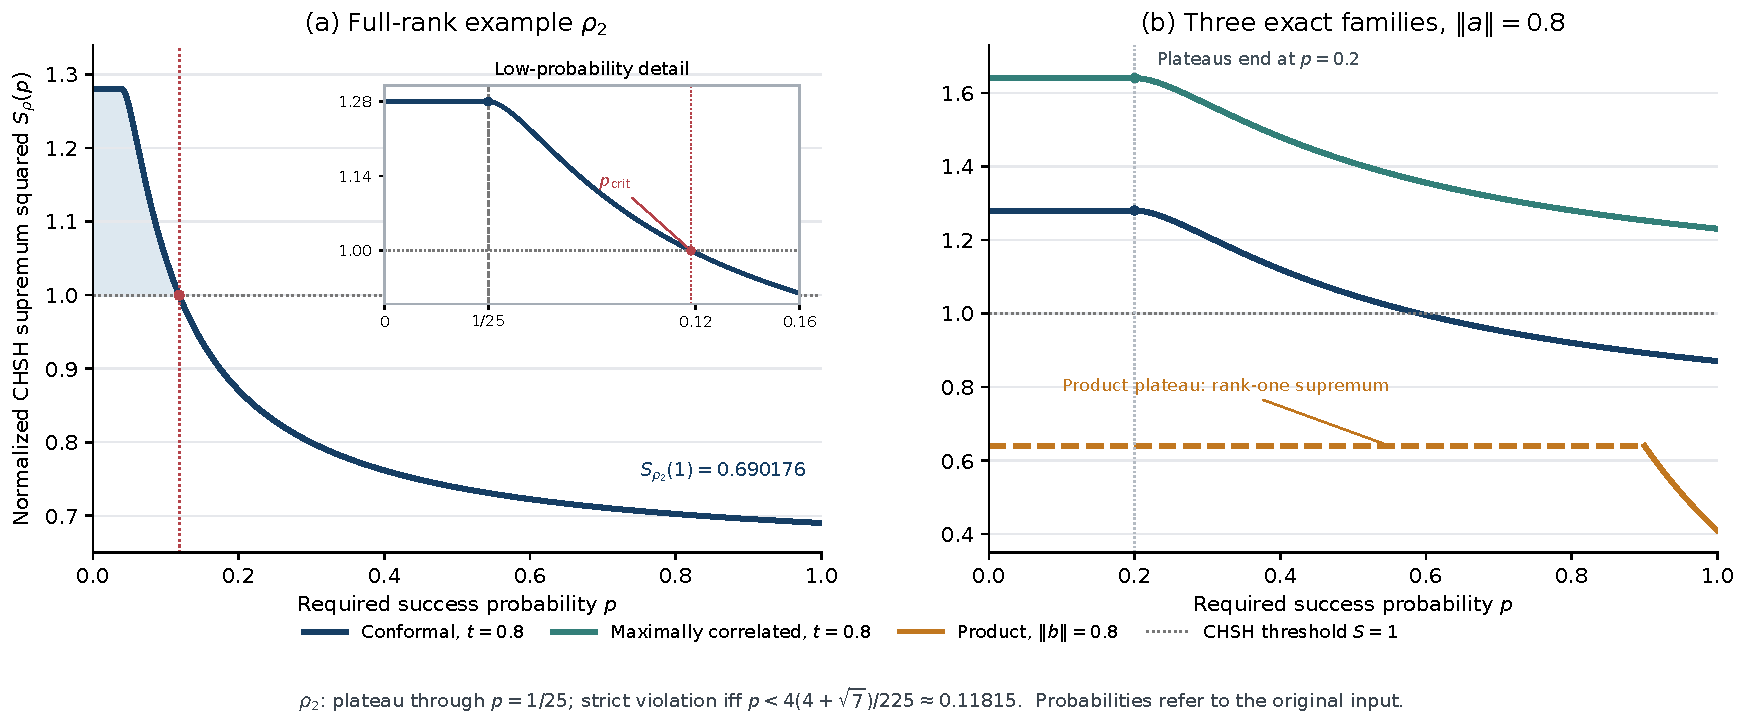
\includegraphics[width=\textwidth]{figures/original_success_frontiers.pdf}
\caption{Exact success frontiers on the original input. The full-rank
$\rho_2$ example violates exactly for required probabilities
$p<4(4+\sqrt7)/225\simeq0.11814669$ and attains its unconstrained score
for $p\le1/25$. The family comparison uses $\norm a=0.8$ and
$t=0.8$ for the conformal and maximally correlated states, and
$\norm b=0.8$ for the product state. The product plateau is a rank-one
supremum; the two entangled-family curves have finite attaining filters.}
\label{fig:r3-frontiers}
\end{figure}
\paragraph{Numerical scope.}
The file \texttt{calculations/original\_input/original\_success.py} evaluates the exact Bob Gram
matrix, projects candidates into the true lens, and performs multistart
optimization over all three effect coordinates. Its general output is
explicitly labeled as a numerical candidate, not a global certificate.
The closed families above and the counterexample are separately checked
using direct complex density matrices and exact symbolic identities.
